\chapter{Integration Engineering}
\label{sec:fdsp-coord-integ-sysengr}
%\chapter{Integration}
%\label{vl:tc-integration}


Integration engineering focuses on configuring the
mechanical and electrical systems of each detector and the interfaces
between them. This includes verifying that subassemblies and their
interfaces are correct (e.g., \dword{apa} and \dword{dsp} \dword{pds}). A
second major focus is supporting the \dwords{detmodule} and their
connections to the cryostat and cryogenics. A third major focus is
assuring that the \dwords{detmodule} can be installed: that the
integrated components can be moved into their final configuration. A
fourth major focus is integrating necessary services provided by
conventional facilities and the \dwords{detmodule}.


The \dword{tc} engineering team maintains configuration data to manage
the detector configuration. The consortia provide engineering data for
their subsystems to \dword{tc}. The \dword{tc} engineering team will
work with the \dword{lbnf} project team to integrate all detector data
into the global \dword{lbnf} configuration files.  These tasks use the
tools and practices described in the rest of this chapter.


\section{Integration Models}
\label{sec:fdsp-coord-integ-models}

The \dword{dsp} and \dword{ddp} detectors are large and are made of many
intricate components. Fortunately for the most part, the
components are repetitive and not overly complex
geometrically. Thus, 3D mechanical modeling techniques are well suited
to represent the detectors and manage their configuration.

At the same time, 3D modelling techniques vary in the way items are
represented and in the way the techniques are carried out. Thus, a set
of 2D integration drawings must be generated; these drawings must be
clear and unambiguous across the collaboration. Such 2D drawings are
the basis for the 3D models as well as the basis of the engineering
design of all components.


\subsection{Static Models}
\label{sec:fdsp-coord-integ-static}

\dword{tc} generates and maintains 3D detector
integration models as well as 2D integration drawings. These models
are static because they represent all components at their design
dimension. They do not represent effects of gravity, tolerances, cold
temperature and installation and assembly clearances.


The 3D models are assembled by combining component models from various
consortia. The 3D model files are shared with the consortia in
read-only files. The 2D integration drawings, which are generated from
the 3D models and disseminated, show the interfaces to the level of
detail necessary to ensure proper fit and function. Any issues that
arise are communicated to the consortia, and a resolution method is
determined. The \dword{tc} engineering team will not
change any consortia component models.


The consortia must resolve any issues using agreed upon methods and
provide updated models for reintegration. Using this process, models
are kept synchronized with integration occurring in only one
direction; only the consortia will modify models.


The level of detail in a model is managed actively because too much detail leads to large file sizes when models are combined and
then incorporated into global models of facilities. The \dword{tc} engineering team must ensure the
appropriate level of detail at each stage of model
integration.


Figure~\ref{fig:dune-sp_overall} shows the overall model of the \dword{dsp} far detector. One wall of the cryostat is removed, so the interior
components are visible. The detector has 25 rows, all of which follow
the same construction. At the ends of rows one and 25, end
walls are installed to close the detection volume.
\begin{dunefigure}[Overall model of the single phase detector]{fig:dune-sp_overall}
  {Overall model of the single phase detector.}
  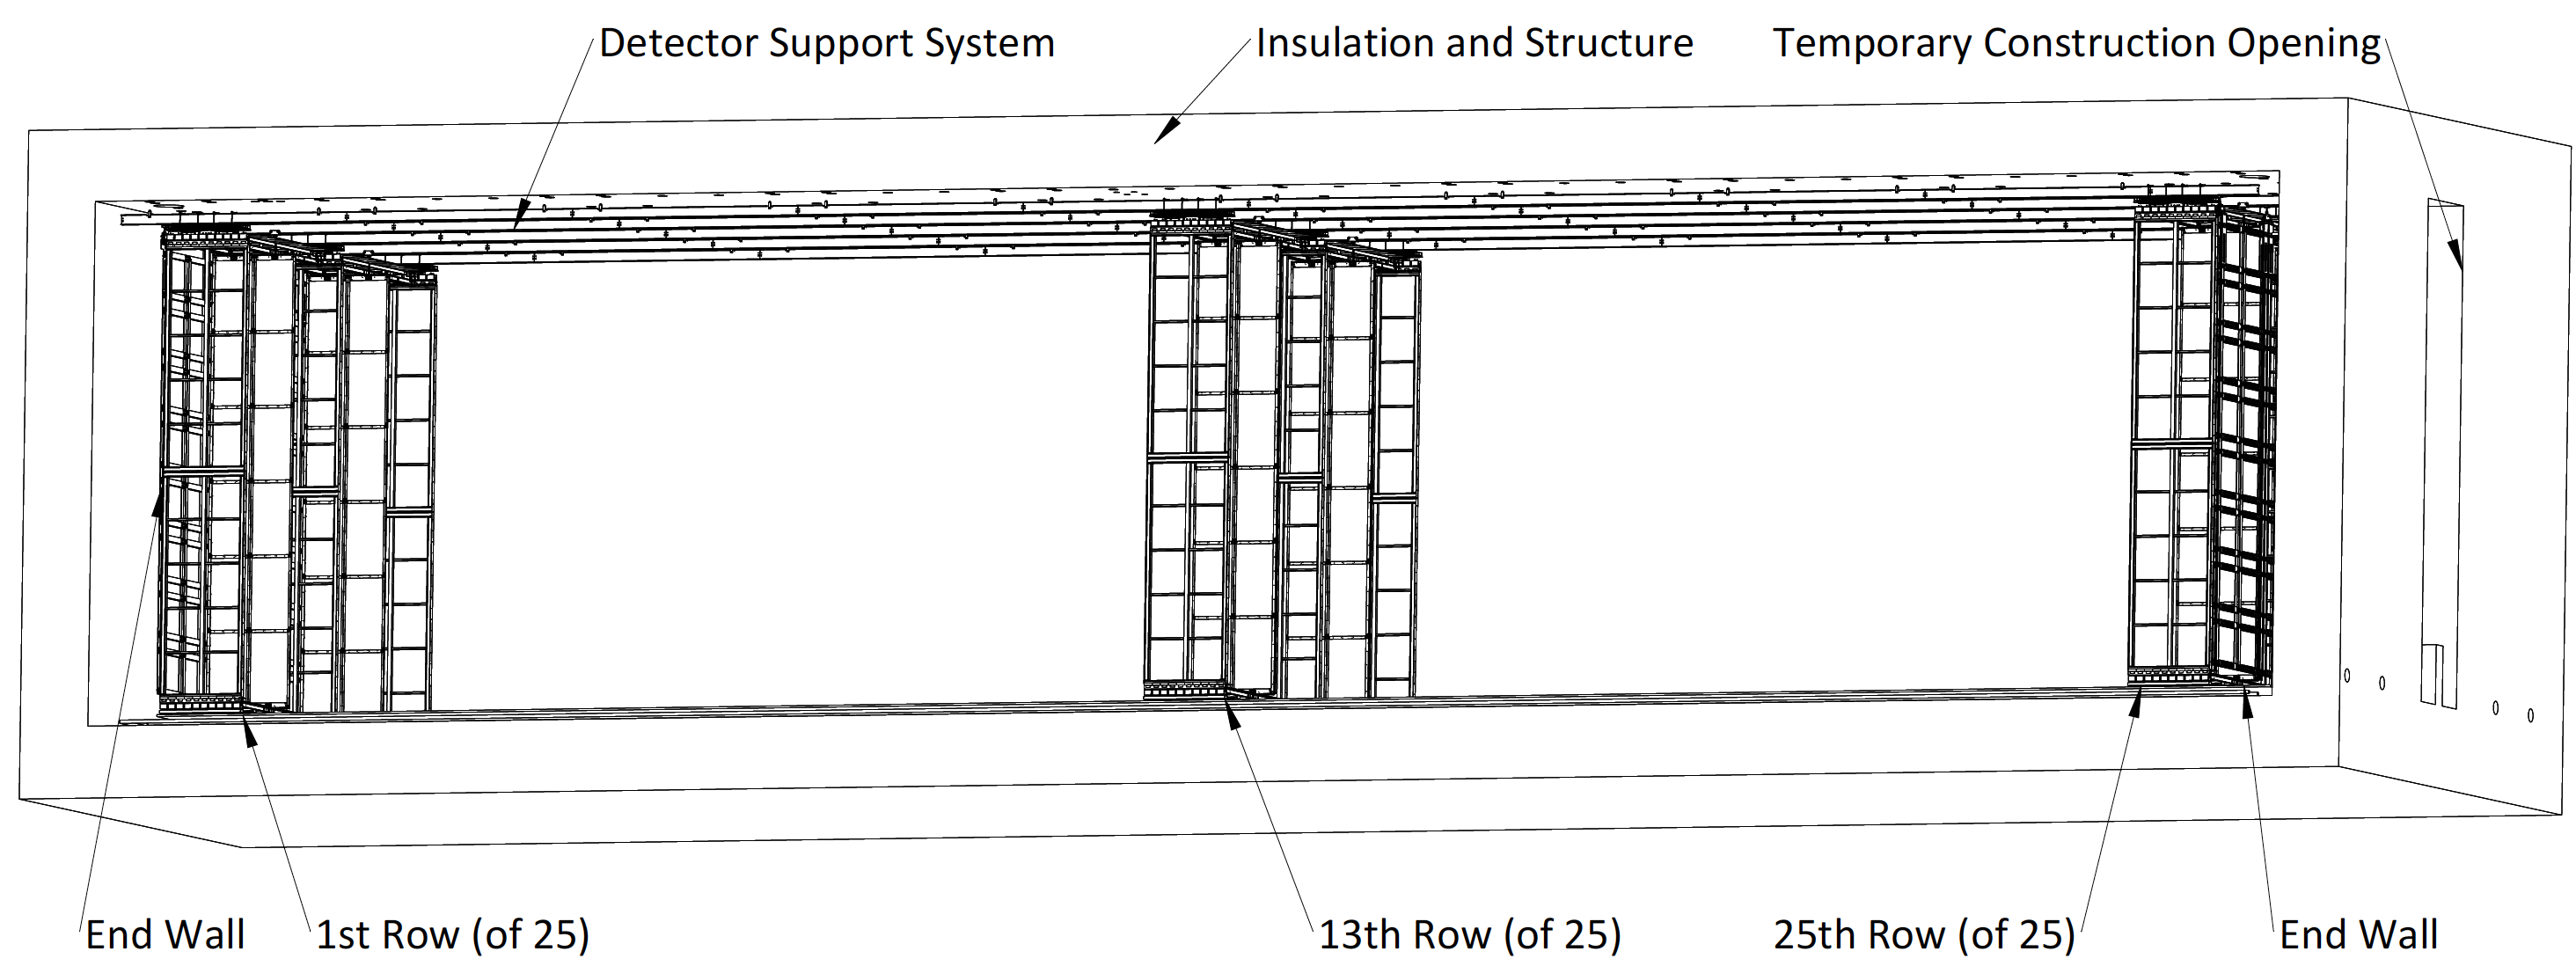
\includegraphics[width=0.85\textwidth]{Overall_model_SP}
\end{dunefigure}
As mentioned earlier, this model does not include all the details of
the detector components. The components are simplified to keep the
overall model complexity to a manageable level.


Figure~\ref{fig:dune-sp_row} shows the model of one row of the
detector module. Each row is constructed from six \dwords{apa}, four
\dwords{cpa} and eight \dwords{fc} and \dwords{gp}. A total of 25 rows
comprise one \dword{dsp} far detector.
\begin{dunefigure}[Overall model of one row of the single phase detector]{fig:dune-sp_row}
  {Model of one row of the single phase detector.}
  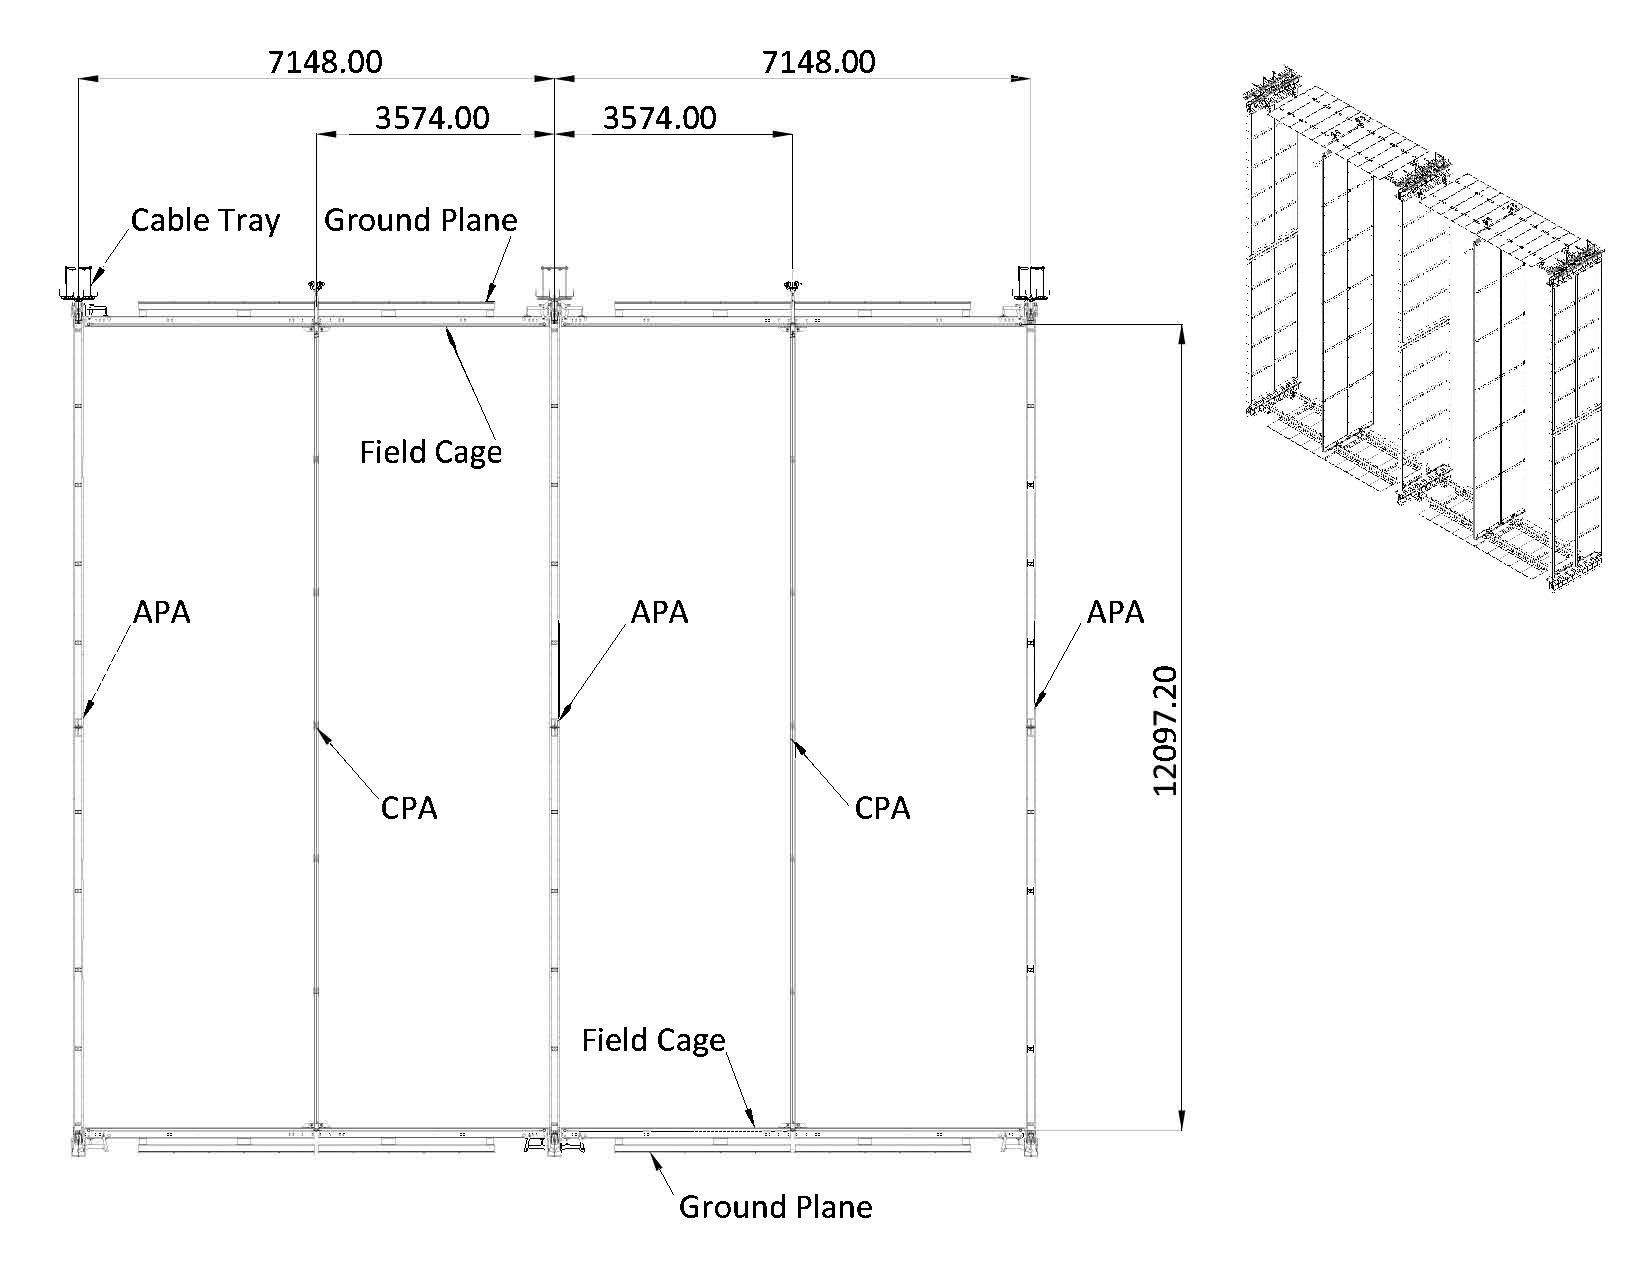
\includegraphics[width=0.6\textwidth]{Model_one_row_SP.pdf}
\end{dunefigure}




Figure~\ref{fig:dune-sp_transverse} shows a cross section of the
\dword{dsp} far detector in the transverse direction and the overall
dimensions.
\begin{dunefigure}[Section view of the single phase detector in the
    transverse direction.]{fig:dune-sp_transverse}
  {Section view of the single phase detector in the transverse
    direction.}
  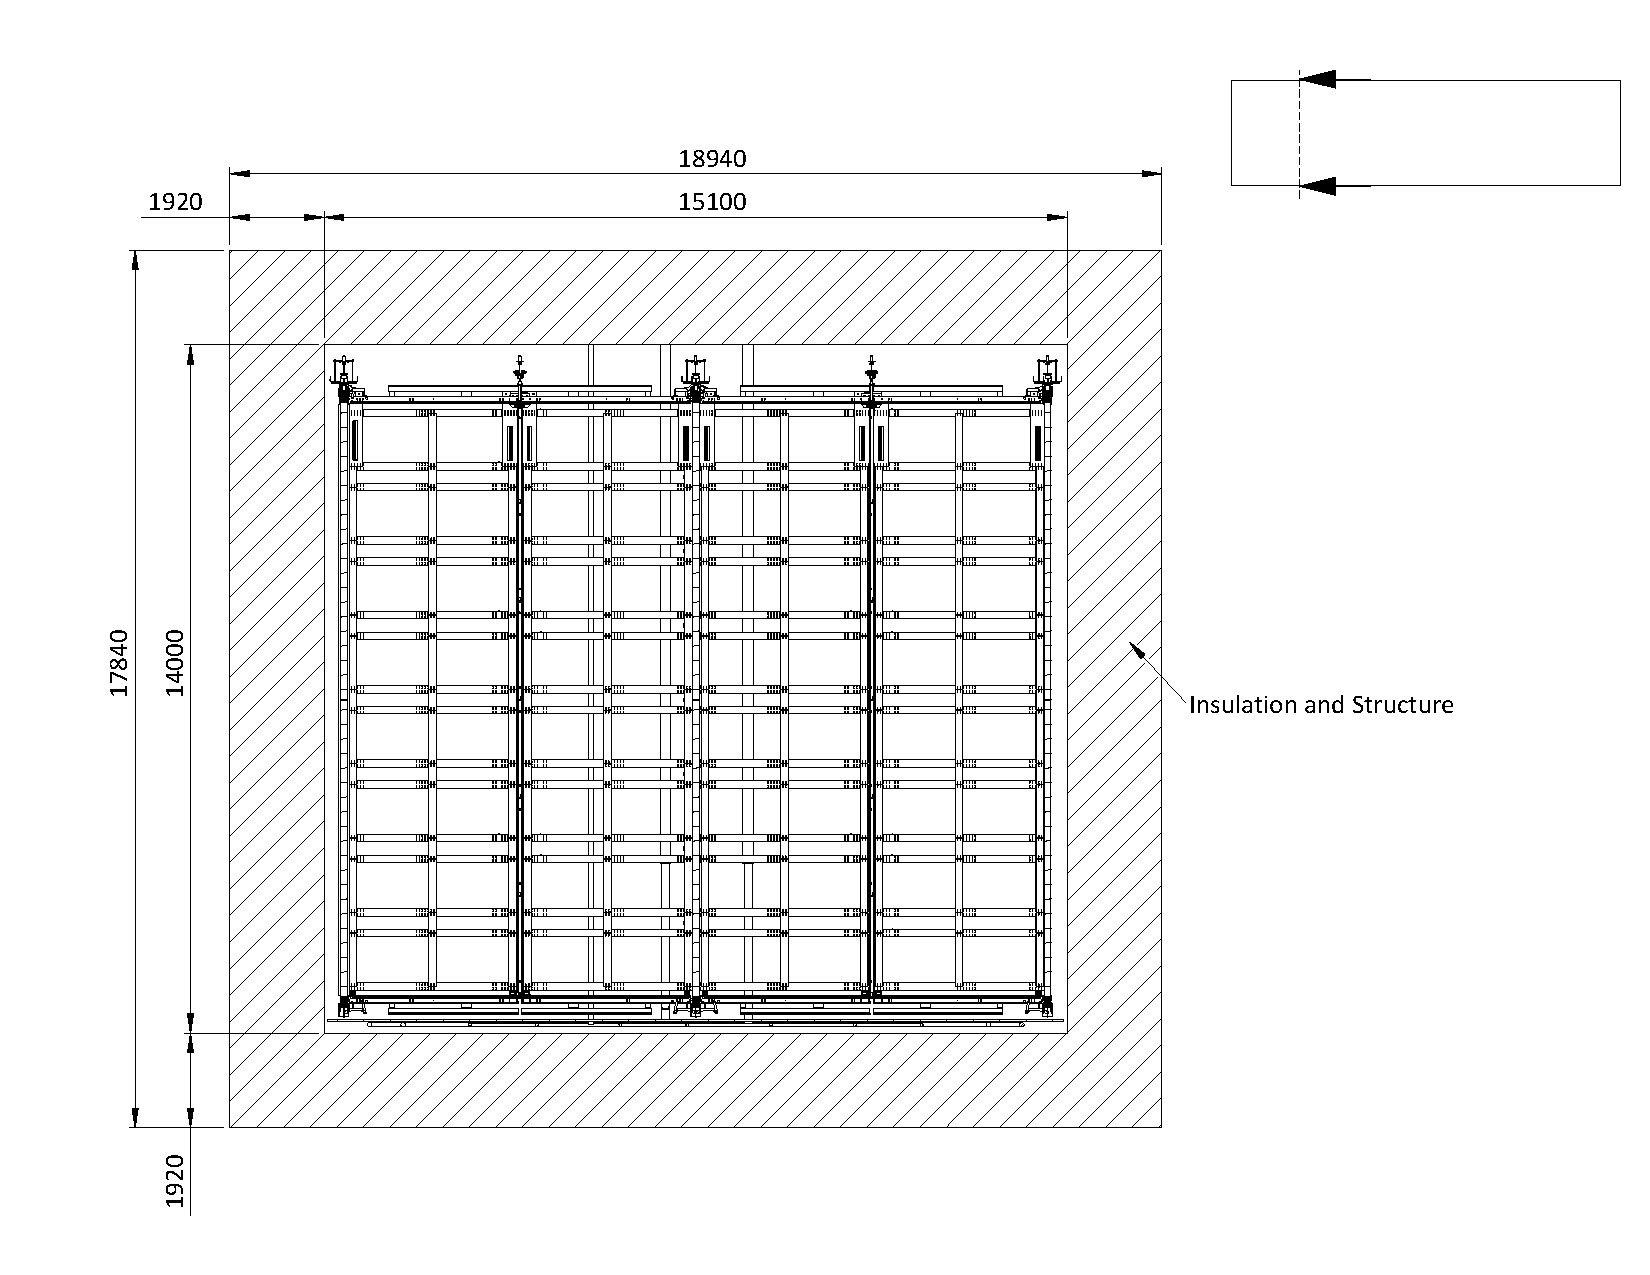
\includegraphics[width=0.55\textwidth]{SP_transverse_section.pdf}
\end{dunefigure}
Figure~\ref{fig:dune-sp_long} shows a cross section of the
\dword{dsp} far detector in the longitudinal direction and the overall
dimensions.
\begin{dunefigure}[Overall model of the Single Phase Detector in the
    longitudinal direction]{fig:dune-sp_long}
  {Overall model of the Single Phase Detector in the longitudinal direction.}
  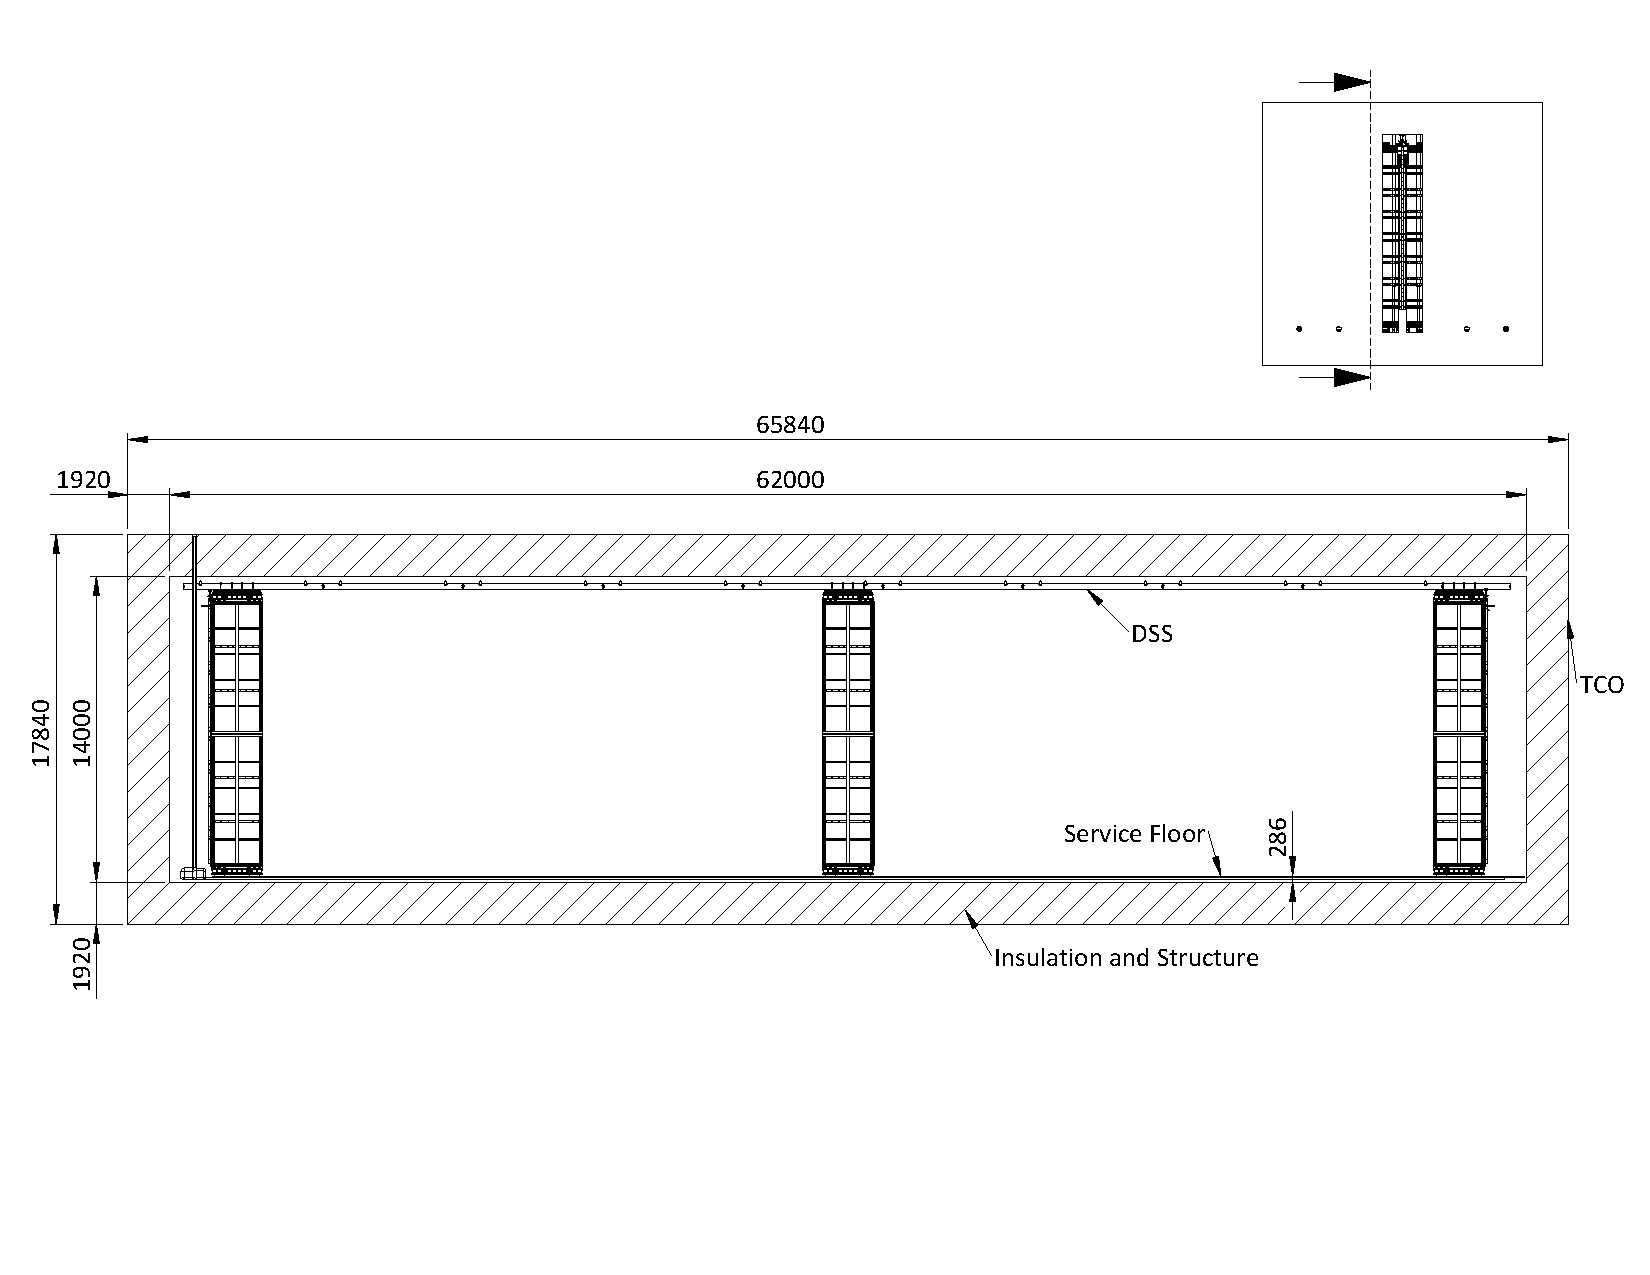
\includegraphics[width=0.85\textwidth]{SP_longitudinal_section.pdf}
\end{dunefigure}


(Note: Need analogous figures and explanations for Dual Phase)


Figure~\ref{fig:dune-dp_overall} shows the overall model of the dual
phase detector, \dword{ddp}. One wall of the cryostat is removed to show
the interior components. The detector has 20
rows, all of which are constructed the same. Each row comprises four
\dwords{crp}, cathode, \dword{gp}, \dwords{pmt} and side-wall \dwords{fc}. 
At the
end of row one and row 20, end walls are installed which close the
detection volume.
\begin{dunefigure}[Overall model of the Dual-Phase Detector]{fig:dune-dp_overall}
  {Overall model of the dual phase detector.}
  \fbox{\parbox[c][6cm]{6cm}{
      \begin{center}
        Dummy Dual-phase figure
      \end{center}
  }}
  %  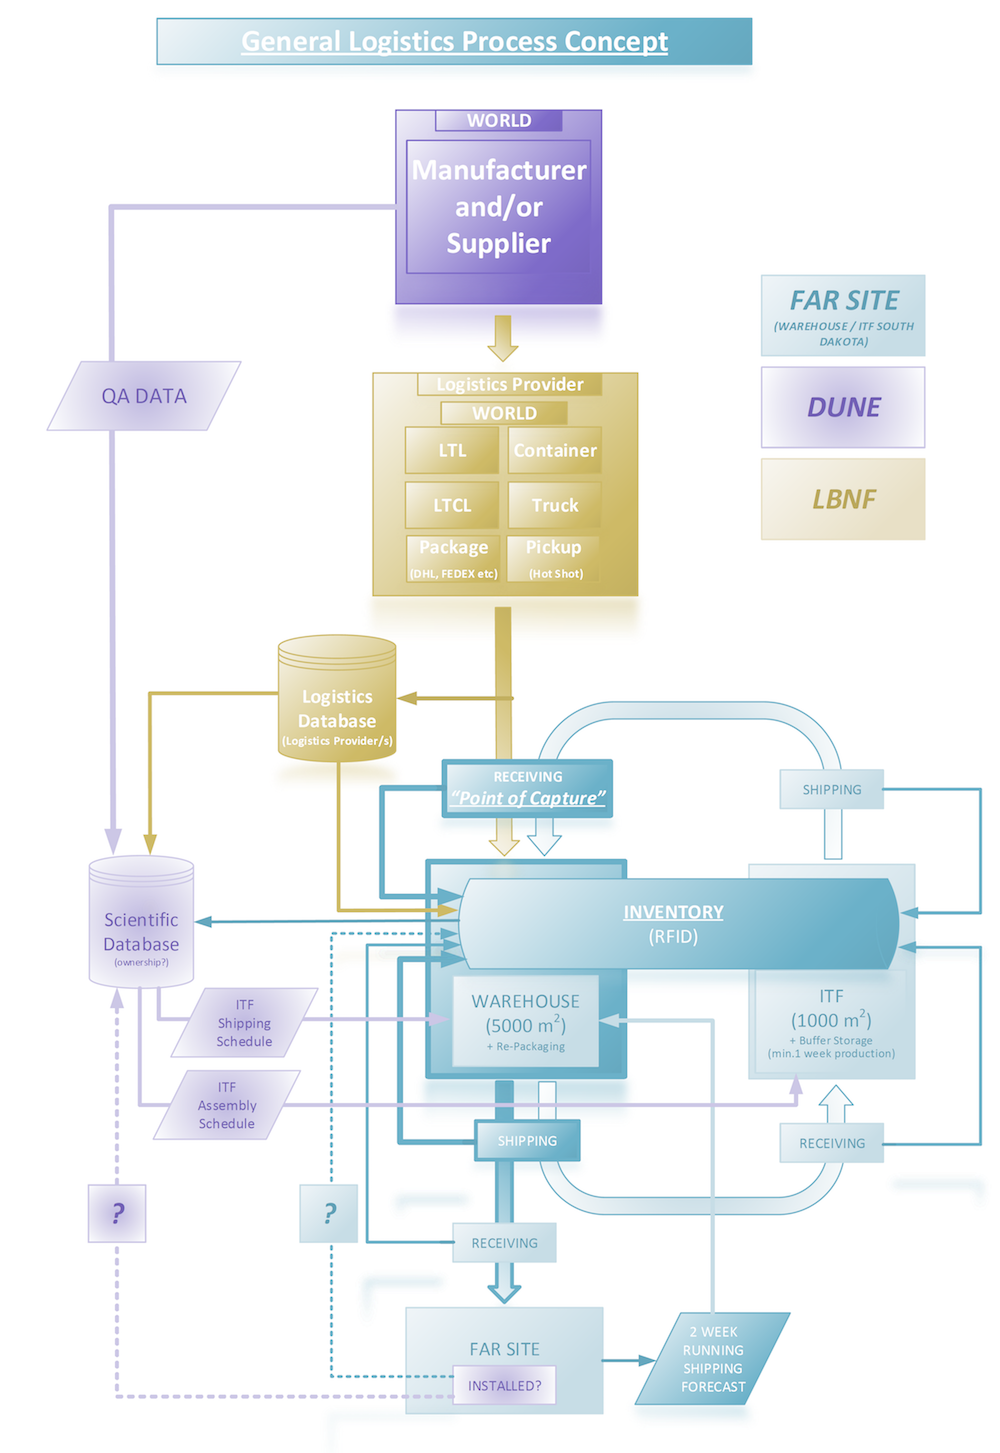
\includegraphics[width=0.85\textwidth]{logistics}
\end{dunefigure}


More detailed models of the \dword{ddp} detector integration
inferfaces are shown in the following figures.


\subsection{Envelope and Assembly Models}
\label{sec:fdsp-coord-integ-envelope}

Static models represent the detector and its components using their exact
design dimensions. Such exact dimensions are needed so the
detail component drawings and model are completely compatible at all
times.


For installation and operation, however, other, more approximate, envelope models are needed. Envelope models will be developed
to address issues that affect installation and operation:
\begin{enumerate}
 \item Effects on the detector caused by distortion of the cryostat
   and detector support structure due to gravity
 \item Effects on the detector caused by distortion of the cryostat
   and detector support structure due to loads on the cryostat during detector filling and operation
 \item Effects on the detector caused by thermal contraction during
   detector filling and operation
 \item Effects of component and
   assembly tolerances
 \item Clearances needed for installation and envelopes needed for
   access and tooling
 \item Reference models and drawings needed for installation stages
   and to control assembly
 \item Reference models and drawings needed for alignment and survey
\end{enumerate}


The models and drawings described above will be generated from static
models. Models will also be generated to
represent combined effects of the above. In all cases, as with static models, 2D
drawings will be created to provide the basis for the installation
drawings.


Generating envelope models and drawings are the responsibility of the
\dword{tc} engineering team in coordination with consortia.




\section{Plan for Model and Drawing Storage and Dissemination}
\label{sec:fdsp-coord-integ-modelplan}

The consortia and \dword{tc} engineering team create and share
drawings, models, schematics, production data and all other
engineering documents. In addition, the \dword{tc} engineering team
generates and shares all interface drawings and documentation.


Folders have been set up that allow uploading and sharing
documents with appropriate protection. The structure of the folders
has been set up to suit each consortium. The
consortia do not necessarily have similar folder structures or files and will adapt
the structure to fit their needs.


The folders and files reside on the \dword{edms}. This system and
similar structures were used for \dword{protodune} and are being
used by \dword{lbnf}.


The following shows a high-level outline of the file structure. The
first section is for technical coordination files. The second
section is generic, intended for a consortium. Each consortium will have one such
folder.
\begin{enumerate}
 \item Technical Coordination
 \begin{enumerate}
  \item Mechanical drawings and files (controlled by the lead mechanical engineer of \dword{dune})
  \begin{enumerate}
    \item Far Detector general drawings for illustration (controlled by \dword{tcoord})
    \item 3-D model files of internal detector for periodic upload to global model
    \item 2-D interface drawing files    
    \item Alignment and survey files
    \item Integration test facility files
    \item Ash River installation test facility files
    \item \dword{qa}/\dword{qc} files
    \item Safety analysis and documentation
    \item Design reviews
  \end{enumerate}
  \item Electrical and electronics (controlled by lead electrical engineer of \dword{dune})
  \begin{enumerate}
    \item Infrastructure requirements for grounding
    \item Consortia interface drawings
    \item Detector electronics grounding guidelines
    \item Detector safety system
    \item \dword{qa}/\dword{qc} files
    \item Safety analysis and documentation
  \end{enumerate}
 \end{enumerate}
 \item Consortia files (One per consortium, controlled by consortia technical leads)
 \begin{enumerate}
   \item 3-D Model files
   \item 2-D Part drawing files
   \item Production files
   \item General grounding diagrams
   \item System level block diagrams
   \item System level wiring diagrams
   \item Software and firmware plans
   \item Custom components, such as ASICs (one folder per component)
   \item PCB components (one folder per component)
   \item Cable components (one folder per component)
   \item Power supply components (one folder per component)
 \end{enumerate}
\end{enumerate}
(Note: add figure once the \dword{edms} structure is set up)


\section{Integration Drawings}
\label{sec:fdsp-coord-integ-drawings}

Within each detector, components from various consortia are assembled
and installed. The interfaces among components are developed and
managed through models and drawings as described in
Section~\ref{sec:fdsp-coord-integ-models}. Many such interfaces must
be controlled. The following section shows some of the interfaces,
controlling dimensions, and configurations.


Figure~\ref{fig:dune-apa_interfaces_top} shows the interfaces for the
top \dwords{apa} in the upper corner of the cryostat. It also shows the position
of the cable penetration for the \dword{apa}. Interfaces with cryostat
corrugations and \dword{lar} fill lines are also shown. The reference plane,
which is defined as the plane of the \dword{apa} yokes is explained in the
alignment section.
\begin{dunefigure}[Interface between upper \dword{apa},
    \dword{fc}, cable trays and \dword{dss}]{fig:dune-apa_interfaces_top}
  {Interface between upper \dword{apa}, \dword{fc}, cable
    trays and \dword{dss}.}
  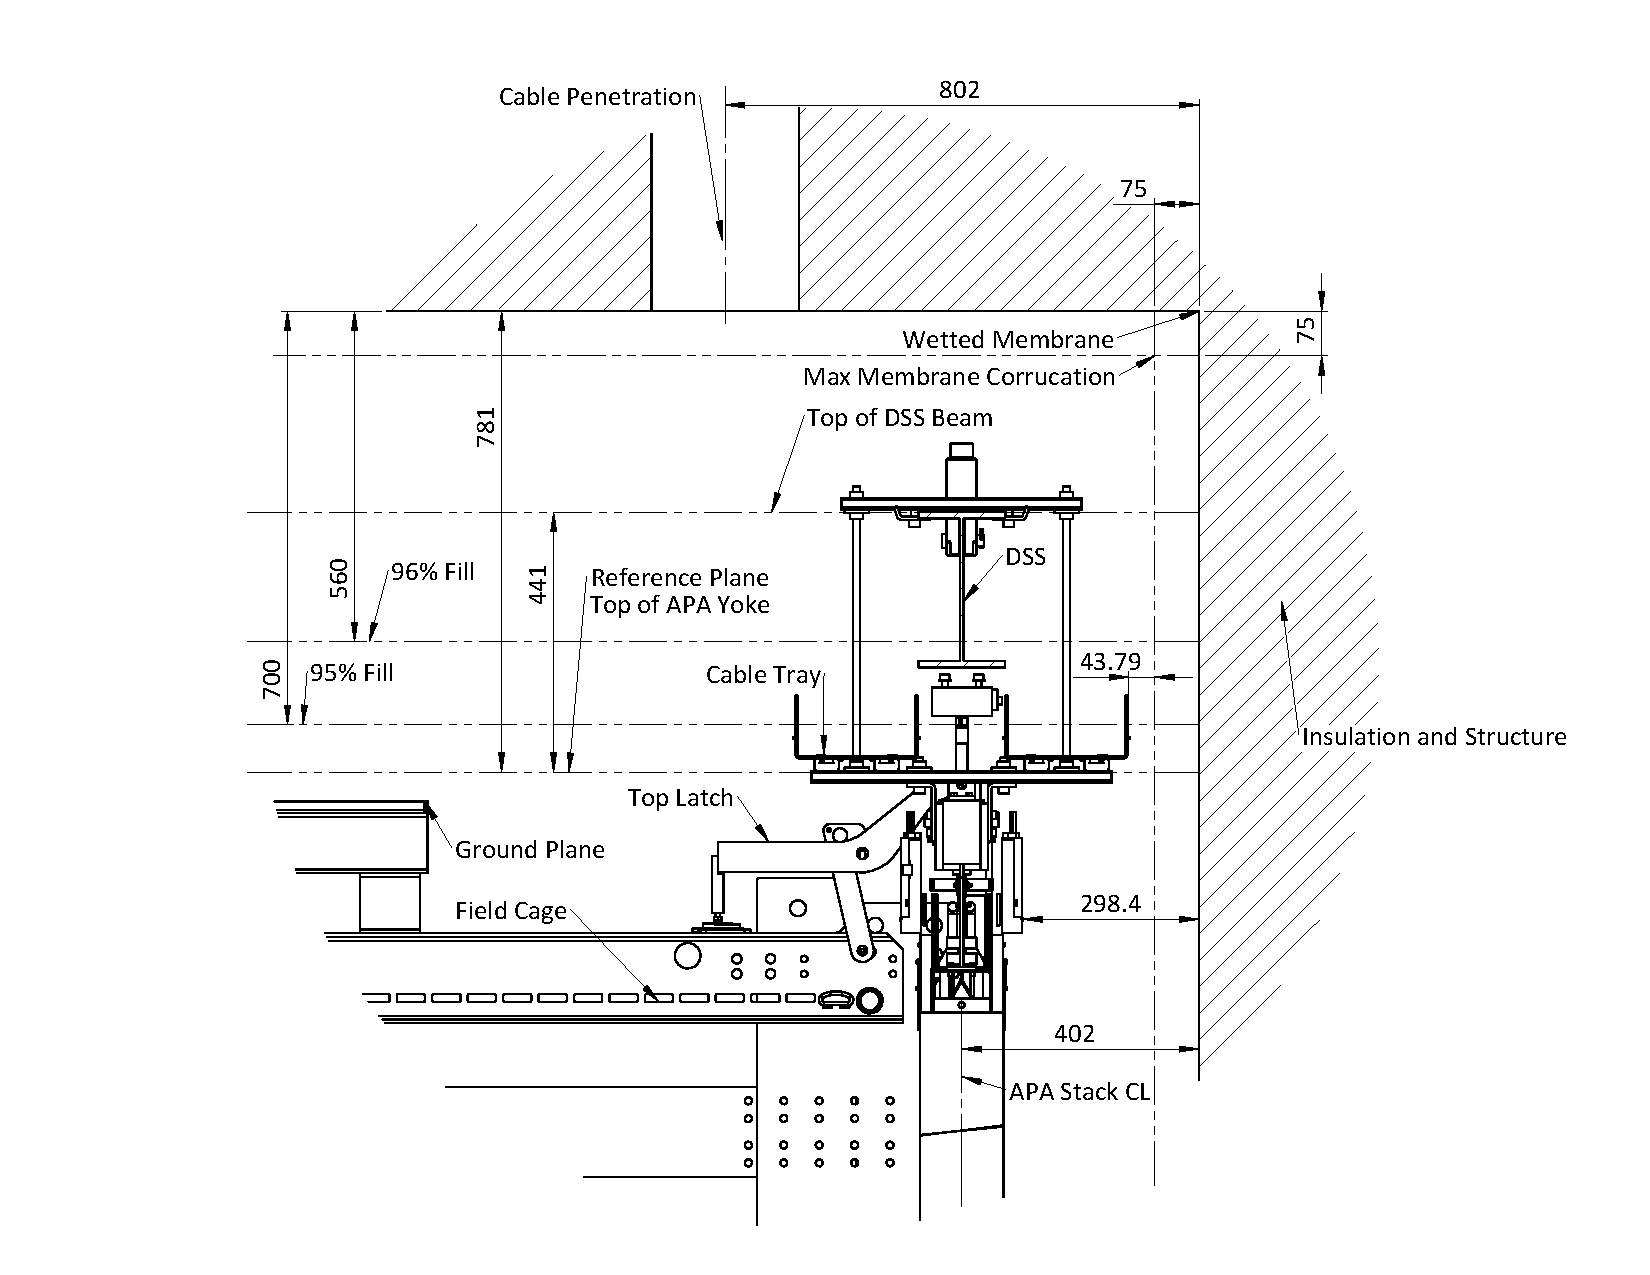
\includegraphics[width=0.7\textwidth]{Interface_upper_apa.pdf}
\end{dunefigure}


Figure~\ref{fig:dune-apa_interfaces_bottom} shows the interfaces for
the bottom \dwords{apa} in the lower corner of the cryostat. In both figures,
the connection latch between the \dwords{fc} and \dwords{apa} is also
shown.
\begin{dunefigure}[Interface between lower \dword{apa}, \dword{fc}
    and service floor]{fig:dune-apa_interfaces_bottom}
  {Interface between lower \dword{apa}, \dword{fc} and 
    service floor.}
  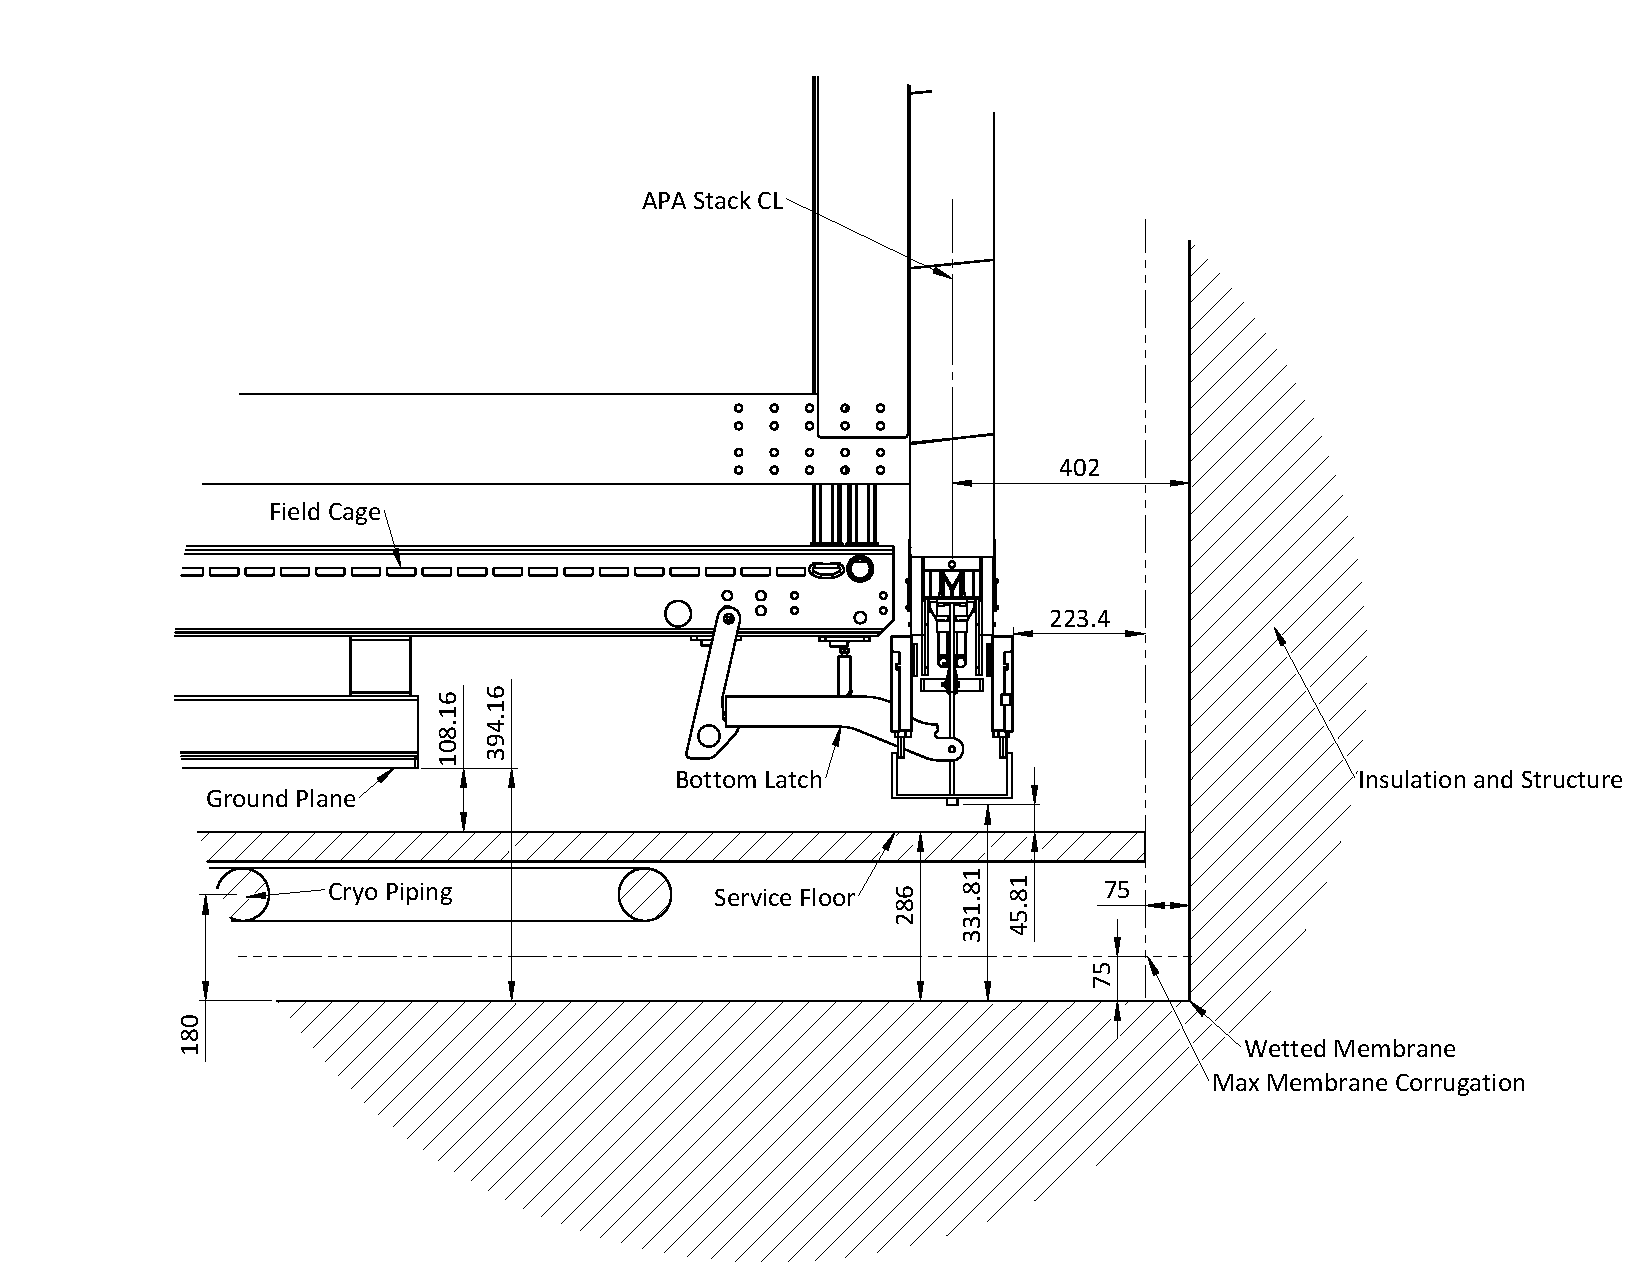
\includegraphics[width=0.7\textwidth]{Interface_lower_apa.pdf}
\end{dunefigure}


Figure~\ref{fig:dune-apa_interfaces_mid} shows the interfaces for the
top of the central row of \dwords{apa} with other components. In this case, a
double latch connection is used. Similarly,
Fig~\ref{fig:dune-cpa_interfaces} shows the interfaces for top of the
\dwords{cpa} with other components.
\begin{dunefigure}[Interface between \dword{apa}, upper \dword{fc} 
    and \dword{gp}]{fig:dune-apa_interfaces_mid}
  {Interface between \dword{apa}, upper \dword{fc} and \dword{gp}}
  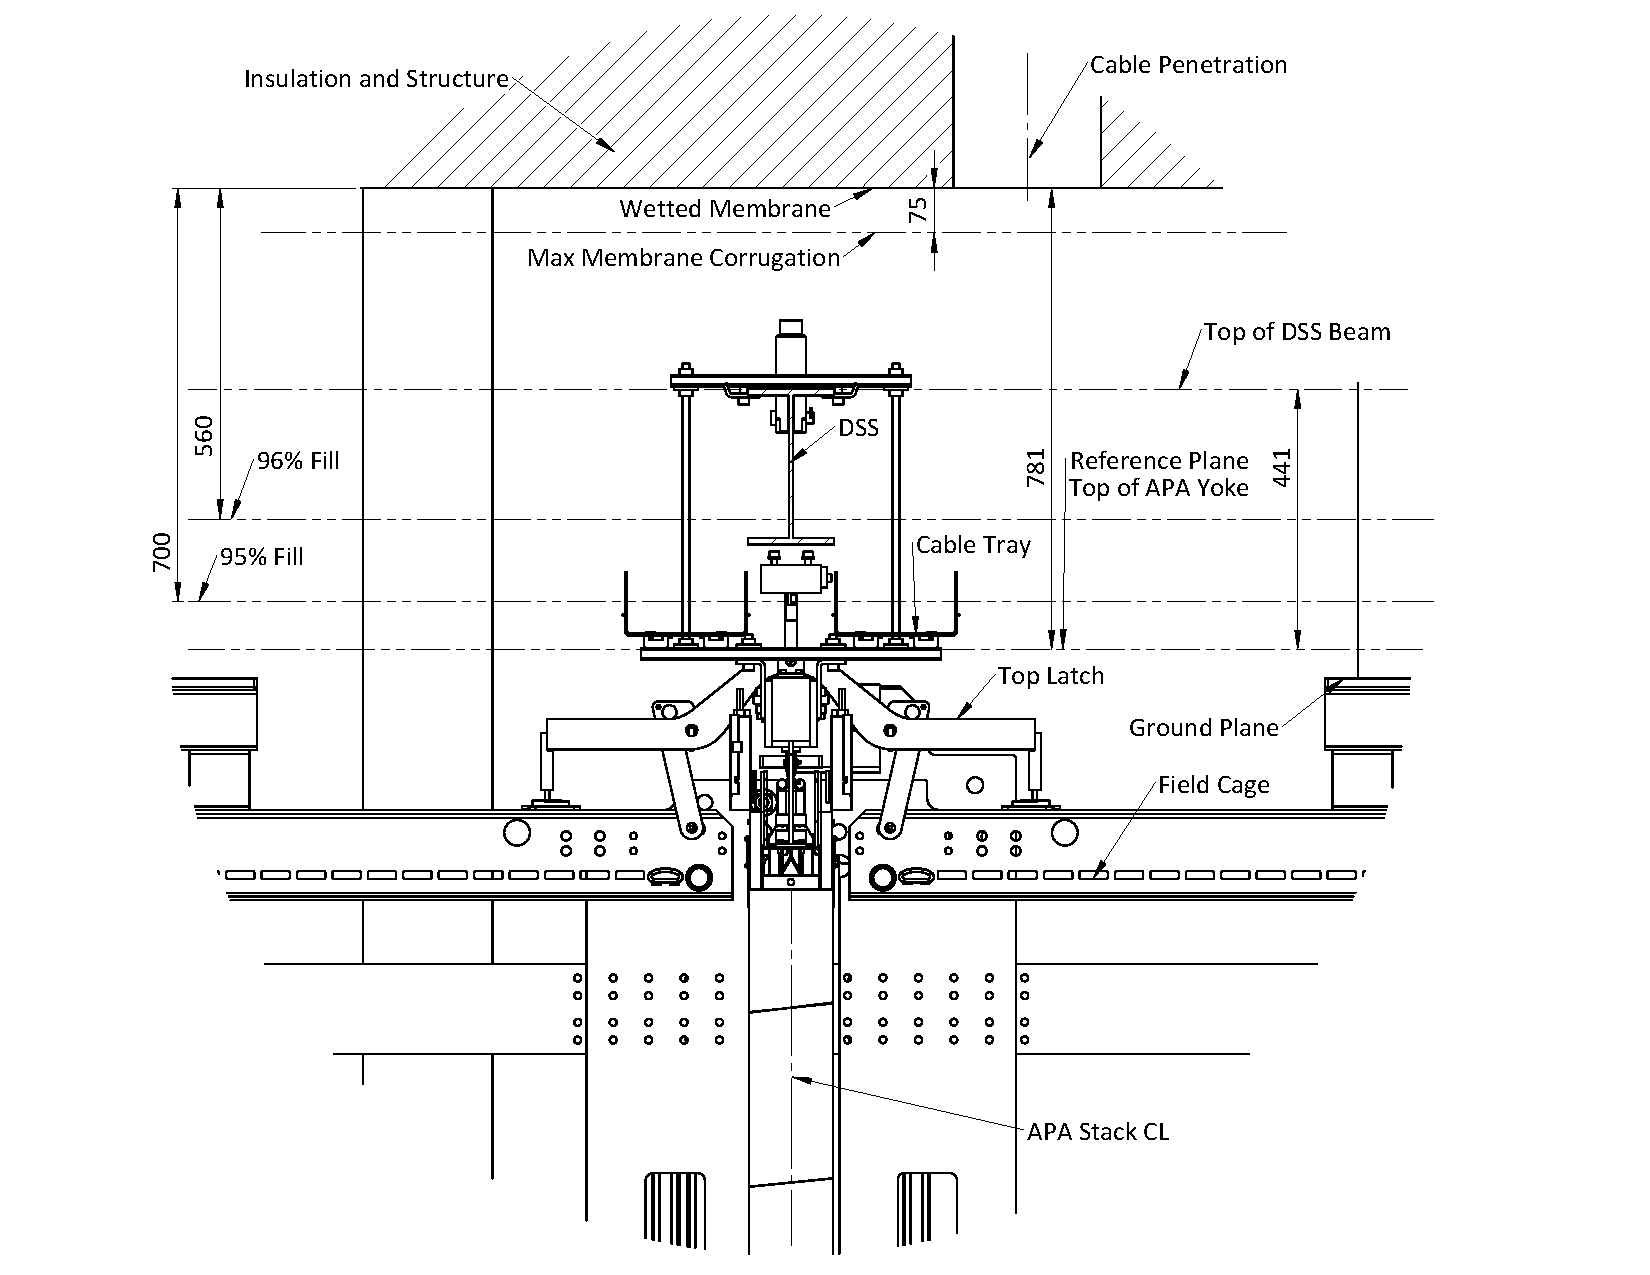
\includegraphics[width=0.8\textwidth]{Interface_upper_mid_apa.pdf}
\end{dunefigure}
\begin{dunefigure}[Interface between \dword{cpa}, upper \dword{fc} and \dword{gp}]
    {fig:dune-cpa_interfaces}
  {Interface between \dword{cpa}, upper \dword{fc} and \dword{gp}.}
  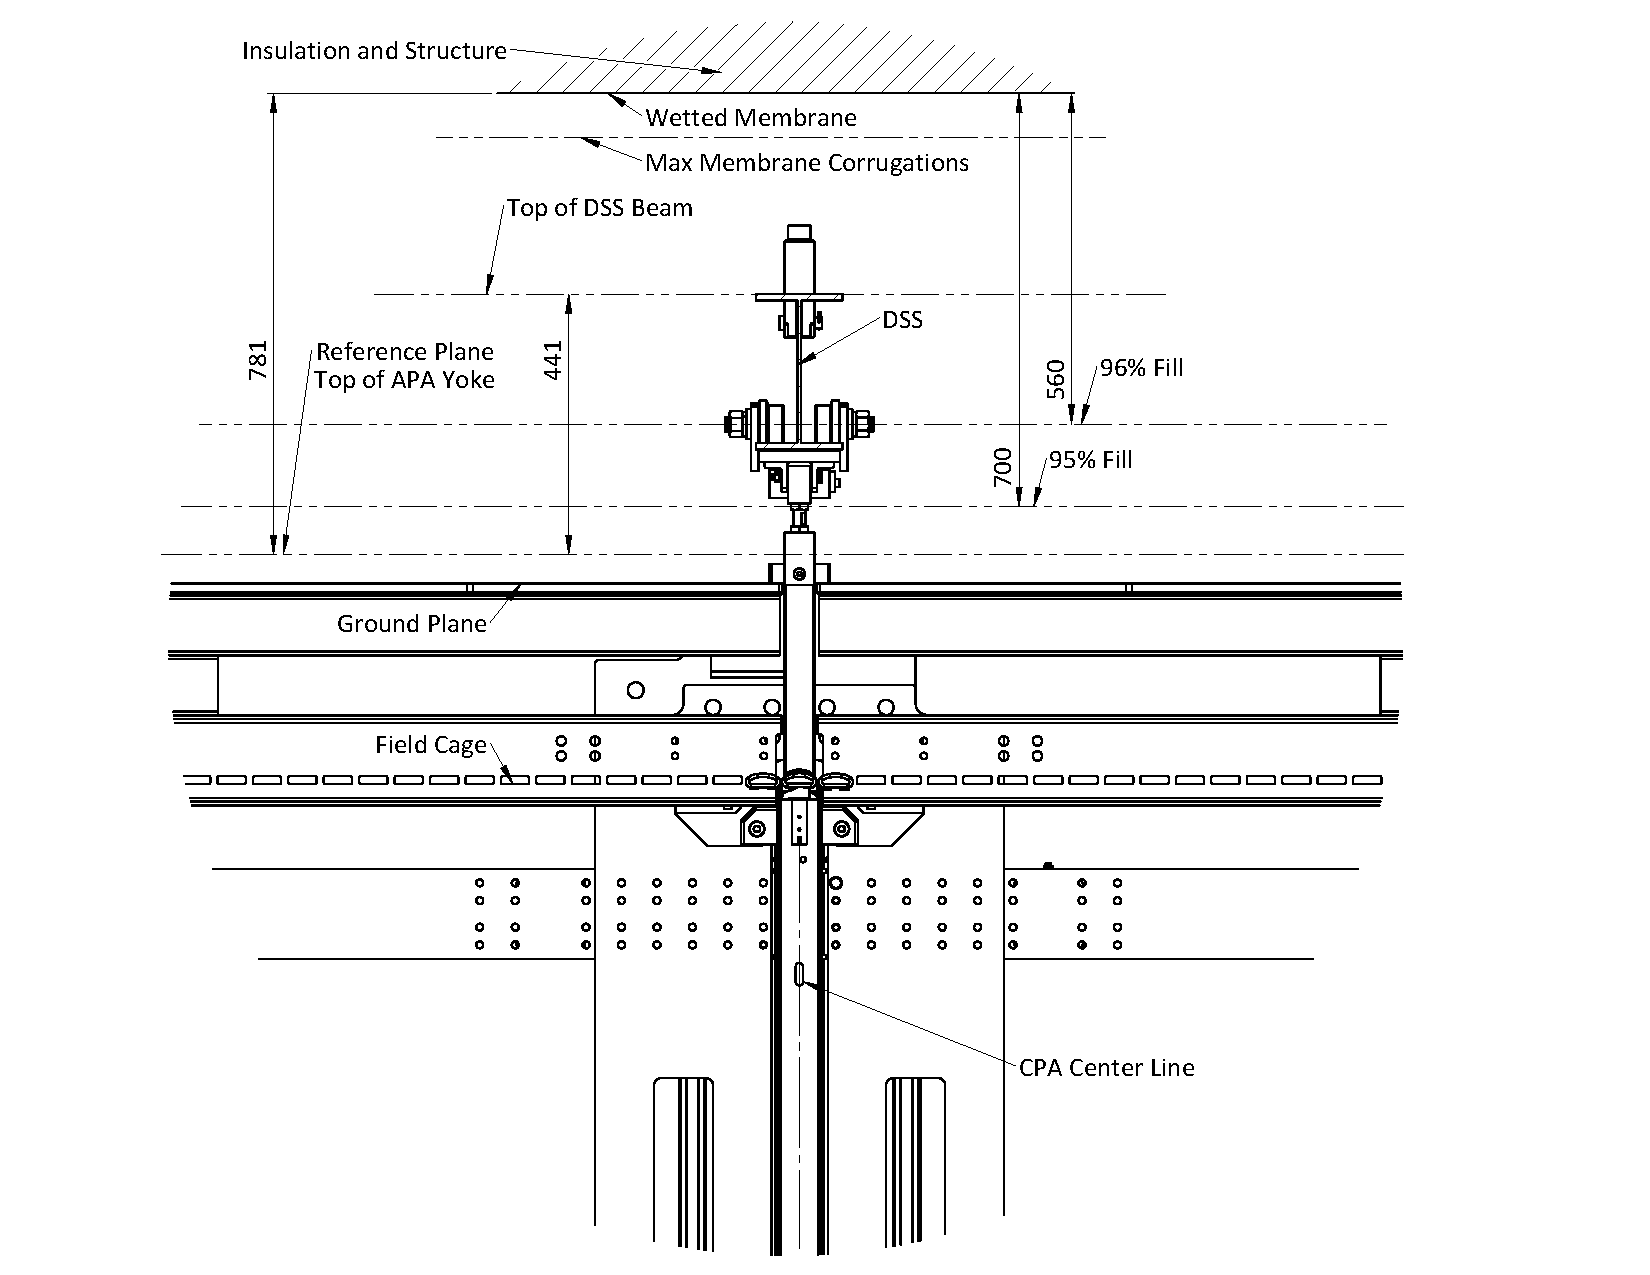
\includegraphics[width=0.8\textwidth]{Interface_upper_cpa.pdf}
\end{dunefigure}

These integration drawings are derived directly from the overall
integration model. The overall integration model is assembled from
component models developed by the consortia. Interfaces are controlled
by \dword{tc} and consortia maintain their model files to be
compatible with the interfaces. During the design phase, models are
assembled and checked continuously. At the time of final design, all
interfaces will be fixed.


Component tolerances and installation clearances are managed through
additional models as described in
Section~\ref{sec:fdsp-coord-integ-envelope}.
Fig~\ref{fig:dune-apa_envelope} shows the \dwords{apa} and
\dwords{cpa} as well as their relieve positions that show how they are
constrained within the detector.
\begin{dunefigure}[Graphical representation of envelope dimensions and
    installation clearances for \dwords{apa} and \dwords{cpa}
    in the warm state]{fig:dune-apa_envelope} {Graphical
    representation of envelope dimensions and installation clearances
    for \dwords{apa} and \dwords{cpa} in the warm state.}
  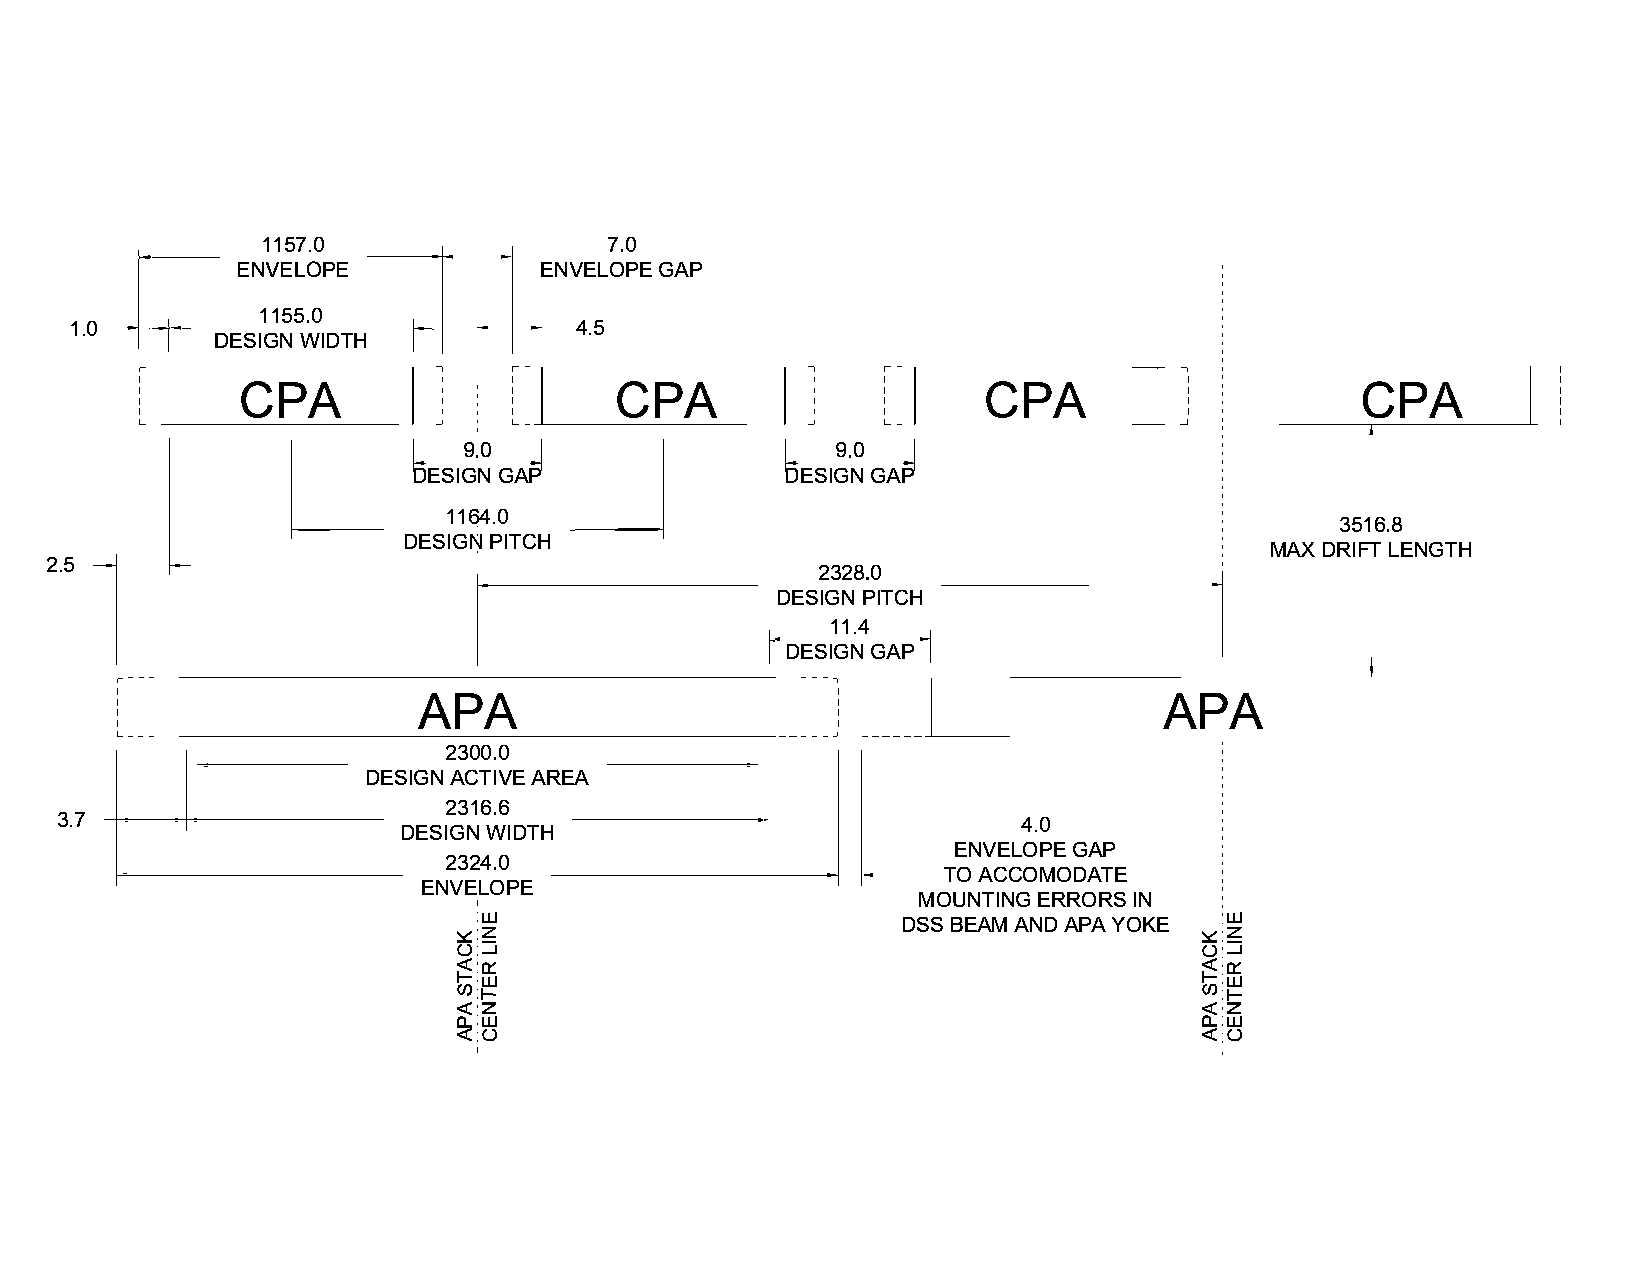
\includegraphics[width=0.95\textwidth]{Warm_envelope_dimensions.pdf}
\end{dunefigure}


This figure shows design dimensions. Component tolerances and assembly
tolerances for the upper and lower \dwords{apa} and \dword{cpa} stacks
have been analyzed and represented as envelope dimensions. An envelope
gap has been defined to account for tolerances in the support system
position and among components. Taking all of these into account, pitch
distances for \dwords{apa} and \dwords{cpa} have been defined in the
warm state.


Figure~\ref{fig:dune-apa_envelope} shows the design drift distance in
the warm state. The drift distance is defined as the perpendicular
distance between the surface of \dwords{cpa} and the collection wire
plane of \dwords{apa}.




\Dwords{apa} and \dwords{cpa} are supported in groups of two or three
on the detector support beams.  In the cold state, the relative
position of groups of \dwords{apa} and \dwords{cpa} change because of
thermal contraction, while relative positions within each group are
relatively constant. Figure~\ref{fig:dune-apa_envelope_cold} is a
graphical representation of the \dword{tpc} in the cold state. 
\begin{dunefigure}[Graphical representation of envelope dimensions and
    installation clearances for Anode Plane and Cathode Plane
    Assemblies in the cold state]{fig:dune-apa_envelope_cold} {Graphical
    representation of envelope dimensions and installation clearances
    for anode plane and cathode plane assemblies in the cold state.}
\end{dunefigure}


The design of the detector support system and the cryostat directly
affect the cold state. The effects of gravity and buoyancy are not
represented either. Such effects are under study and will be shown in
the models as design progress.


Before installing the detector, a set of cryogenic distribution
pipes are installed on the floor of the cryostat. In addition, the
membrane of the cryostat will have corrugations that impede
movement. Therefore, a temporary service floor will be installed. The
floor will be installed, and later removed, in
sections. Figure~\ref{fig:dune-floorpipes} shows this.


\begin{dunefigure}[Interface of cryogenic distribution pipes, service floor and detector.]{fig:dune-floorpipes} 
{Interface of cryogenic distribution pipes, service floor, and detector.}
  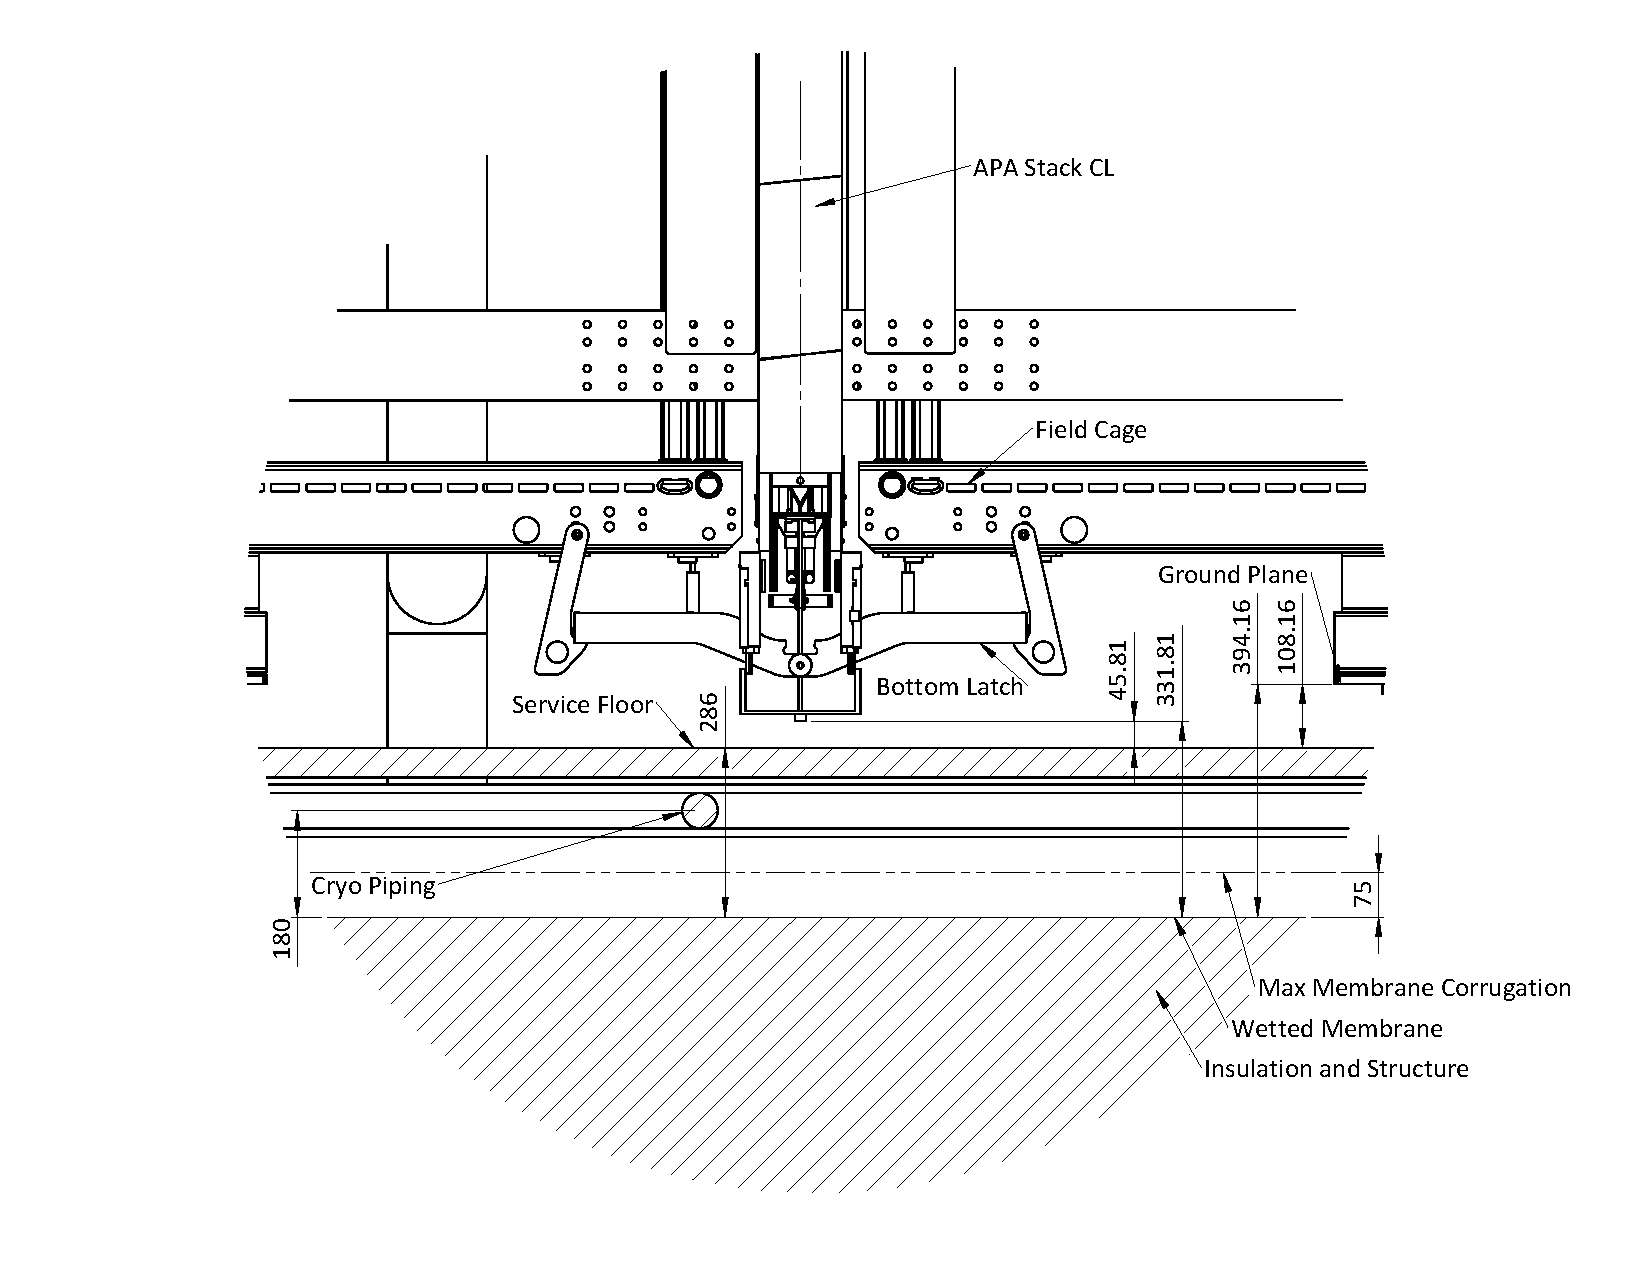
\includegraphics[width=0.8\textwidth]{Interface_lower_mid_apa.pdf}
\end{dunefigure}




(Note: Need analogous figures and explanation for Dual Phase)




\section{Electrical System Block Drawings, Schematics, Layouts and Wiring Diagrams}
\label{sec:fdsp-coord-electrical}


The electrical design of each subsystem is described by a
set of documents that includes a system level block
diagram and one-line power/grounding documentation.
Depending on what is being described, a complete set of schematics,
board production files and wiring diagrams will be reviewed and archived.  All
designs are subject to electrical safety review before
installation and the safety review should begin through
\dword{tcoord} early in the design process.


Consortia will produce system level block
diagrams. \dword{tcoord} will ensure that the
block diagrams are produced and reviewed.  In some cases, multiple
system level block diagrams may be required.  The slow controls consortium is one example of this, with several types of systems (such as \dword{rtd}
readouts, purity monitors, cameras, pressure sensors), each
requiring a separate system level block diagram. A system level block
diagram should show the conceptual blocks required in the design along with connections to other conceptual block elements, both inside and outside the consortium.  
Figure~\ref{fig:electrical_blockdiagram_example} shows an example of a system level block diagram.
\begin{dunefigure}[Example system level block diagram]{fig:electrical_blockdiagram_example}
  {Electrical system level block diagram example (SP cold electronics).}
 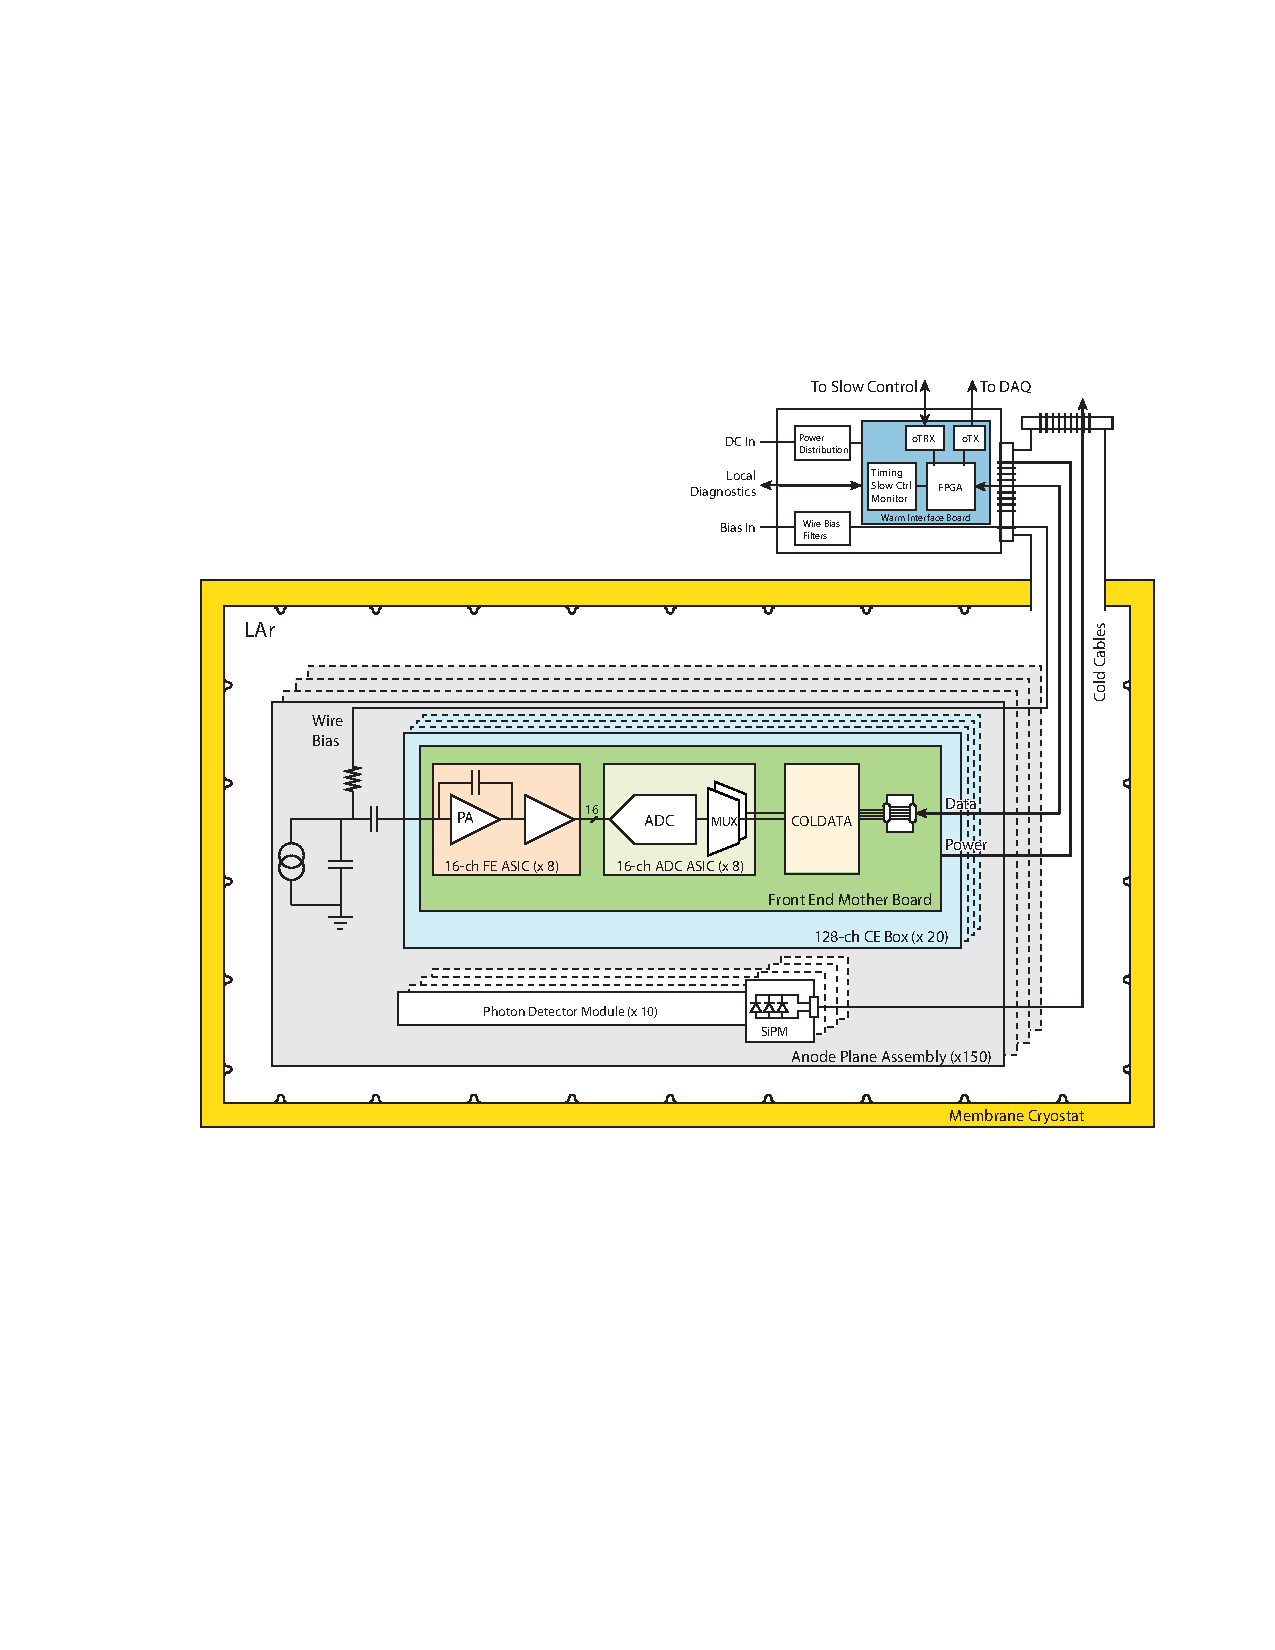
\includegraphics[width=0.85\textwidth]{Example_System_Level_Block-Diagram-SP_Cold_Electronics.pdf}
\end{dunefigure}


An electrical one-line drawing represents the power and ground
distribution within the system being described.  The path of power and
ground distribution wiring between circuit elements are
specified along with wire types and sizes.  Power elements like power supplies, fuses (or other protective circuit elements),
power connectors and pin ampacity are documented.


Electrical schematics show very specifically how individual
components are connected.  Usually, a schematic will represent a
printed circuit board design.  Schematics call out specific
parts that are used in the design and include all interconnections.
In the case of a printed circuit board, layout files, manufacturing
specifications, and bills of materials document
the design and allow a safety review of any custom boards or
modules.


Wiring diagrams include all wire and cable connections that
run between printed circuit boards or electronics modules.  Wires and
cables are described within the diagram and
include identification of wire \dword{awg}, wire color, cable specification
and cable connectors and pinouts.




\section{Electrical Integration Documentation}
\label{sec:fdsp-coord-integ-electrical}

Section~\ref{sec:fdsp-coord-electrical} listed the documentation
required to describe construction of a subsystem corresponding to the
design responsibilities within a consortium.  Interfaces that occur
between consortia subsystems must be documented and formally agreed
upon between the technical leads of the coordinating consortia and
must be verified by the \dword{tcoord} team.  Much of the
documentation required to describe a subsystem is also required for
integration.


Documentation required for the interface between two electrical
subsystems includes a block diagram that identifies all connections
between the subsystems.  This block diagram must exist in the formal
interface document between consortia.  For each connection, additional
documentation must fully describe the interface
details. This additional detailed information can exist outside of the
primary interface document between consortia, but it must be pointed
to within that document.


One example of an integration interface is a signal cable that runs
between printed circuit boards belonging to different consortia.  For
a signal cable, interface documentation include the connector
specifications, pinouts at each end of the cable and the pinout of the
board connectors.  Documentation also describes
relevant electrical signal characteristics that may include signal
levels, function, protocol, bandwidth and timing information.  If
signals are referred to using different signal names between
subsystems, documentation of signal name cross reference must be
provided.


Consortia technical leads and the \dword{tcoord} team must sign off
and approve the detailed documentation information on integration
interfaces not included in the primary consortia to consortia
interface document.




\section{Detector Survey and Alignment}
\label{sec:fdsp-coord-integ-survey}
The detector placement within the cryostat inside the
cavern does not have a physics requirement. The requirement is driven
by overall mechanical assembly needs so that interfacing
parts are assembled properly and function as intended.


In this section, reference frames for the detector are defined so the overall survey and alignment can be done within
the cavern reference frame. (Note: we have not yet defined this.)


For the single-phase detector, a flat and level reference  plane is
defined that is coplanar with the upper \dword{apa} yoke
planes. Thus, 75 yoke planes define this flat and
level reference  plane. This reference plane is set at exactly 781 mm below the
theoretical plane of the cryostat top membrane.


The detector reference plane is coplanar with the upper
\dword{apa} yoke planes because all features, including
the active area, are referenced  to this plane.  Once this reference
plane is defined and established through survey, all vertical
distances within the detector are referenced 
and established relative to this
plane.  Figure~\ref{fig:dune-apa_interfaces_mid} shows the reference
plane in relation to the cryostat top membrane and \dword{dss}.


During installation, the height of the \dword{dss} beams
is set in accordance with this relationship. Adjustments are made in the
\dword{dss} to ensure all the beams are in the
correct plane. The combined effects of gravity, buoyancy, temperature and LAr mass
before and after fill are calculated, and further adjustments are made
to compensate. This will ensure that the detector is as close as
possible to design value after fill.


The transverse position of the detector is constrained to the center
of the cryostat. Thus, the mid-plane of the middle row \dword{apa} is
coplanar with the vertical mid-plane of the cryostat. This
relationship is verified when the \dword{dss} beams and central row of
\dwords{apa} are installed. The outer rows are similarly aligned and
surveyed with the offset as shown in Figure~\ref{fig:dune-sp_row}.
\begin{dunefigure}[Position of feedthrough determining the longitudinal
    reference point of the detector]{fig:dss_feedthru}
  {Position of feedthrough determining the longitudinal reference point of the detector.}
  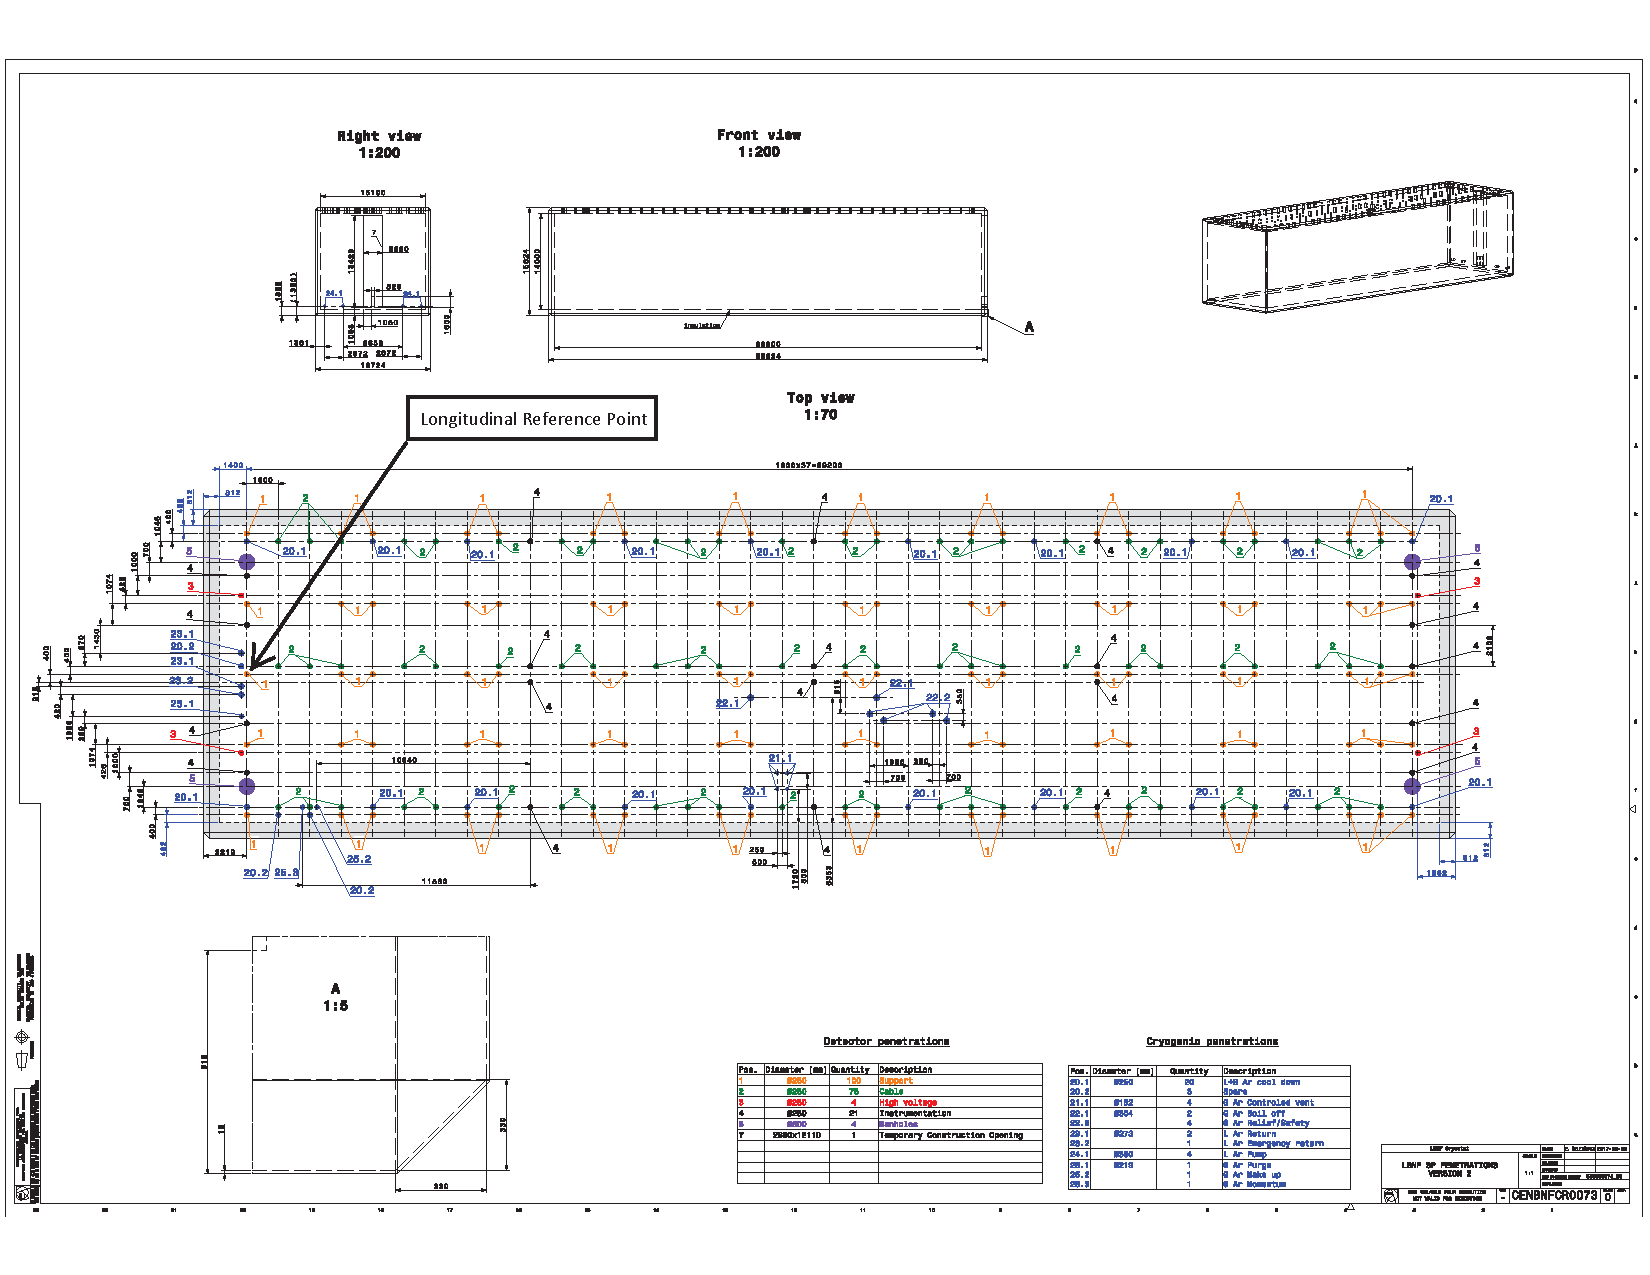
\includegraphics[width=0.9\textwidth]{SP_longitudinal_reference.pdf}
\end{dunefigure}


The longitudinal reference point of the detector within the cryostat
is defined by the position of the single feedthrough of the central row
farthest from the cryostat opening. This feedthrough position
is shown in Figure~\ref{fig:dss_feedthru}.

(Note: The longitudinal position is not fixed at this time. Edit
section as needed once fixed.)


(Note: Dual phase should be similar
transversely and longitudinally, vertically, it needs to be
determined.)


\section{Interface Documents}
\label{sec:fdsp-coord-integ-interface}


Interface documents are developed and maintained to manage the
interfaces among consortia and between consortia and \dword{tcoord}. A
single document covers the interface between any two systems, so any
one system may have several interface documents. If no interface
exists the interface document is not needed. The
interface documents are managed by relevant consortia technical leads
and by \dword{tc} project engineers.

The content of interface documents varies depending on the type
of interface. However, the documents are intended to have
a common structure, defining the interfaces in these sections:
\begin{enumerate}
 \item Definition: This section defines the interfacing systems.
 \item Hardware: In this section, the interfacing hardware components,
   electrical and mechanical, are defined in general terms. As an
   example, the \dword{apa} frame needs to support the \dword{pd} mounting brackets.
 \item Design: In this section, the dependencies in design
   methodology, sequence, and standards are described. As with the
   previous example, the design of the \dword{pd} mounting
   brackets depends on side tubes chosen for the \dword{apa}.
 \item Production: Component production and overall assembly is
   shared among interfacing systems. This section details who has what
   responsibilities.
 \item Testing: Like production, testing is a shared
   responsibility. In this section, responsibilities for testing and
   the required equipment are apportioned.
 \item Integration: The integration of systems into installable units
   before insertion into the cryostat is defined in this section. The
   location, methodology, tooling, and environment for integration are
   defined.
 \item Installation: Installation tasks and responsibilities, once installable units are assembled, are defined in this
   section. Any special transportation or installation tool or fixture
   is also defined.
 \item Commissioning: In this section, overall responsibilities for
   commissioning tasks are defined, and parameters are set.
 \item Appendices: Technical figures and
   interfaces should be included in this section in as much detail as necessary. Block
   diagrams that show interconnections and detailed documentation of
   each connection are needed. 
\end{enumerate}

The interface documents will be developed and modified during the
technical design period. At the time of this writing, not all
documents have been fully developed. Once the technical design is
finished, the interface documents will be placed under revision
control.
